\section{Spannungsausbreitung\label{spannung:section:Spannungsausbreitung}}
\rhead{Spannungsausbreitung}
Anhand untenstehendem Bild kann ein einfaches Beispiel betrachtet werden.
Es gibt eine Flächenlast (Kraft), diese wird auf den Boden abgetragen.
Diese Last muss dann vom Boden aufgenommen werden.
Im Boden entsteht nebst der Eigenspannung eine weitere Spannung durch diese Last (Zusatzspannung).
Diese Zusatzspannung $\sigma$ ist abhängig von $(x,y,t)$.
Je nach dem, wo man sich im Boden befindet variert die Spannung.
Mit der Tiefe wird die Zusatzspannung geringer.
Die Ausbreitung der Zusatzspannung im Boden hat die Form einer Zwiebel.
Durch Untersuchung der Spannung an verschiedenen Punkten im Boden, kann man eine Funktion abtragen.
Dasselbe macht man auch mit der Dehnung. Es zeigt sich, dass die Form der beiden Funktionen gleich ist.
Dies erklärt sich dadurch, dass die Spannung und die Dehnung proportional zueinander sind.
\begin{figure}
	\centering
	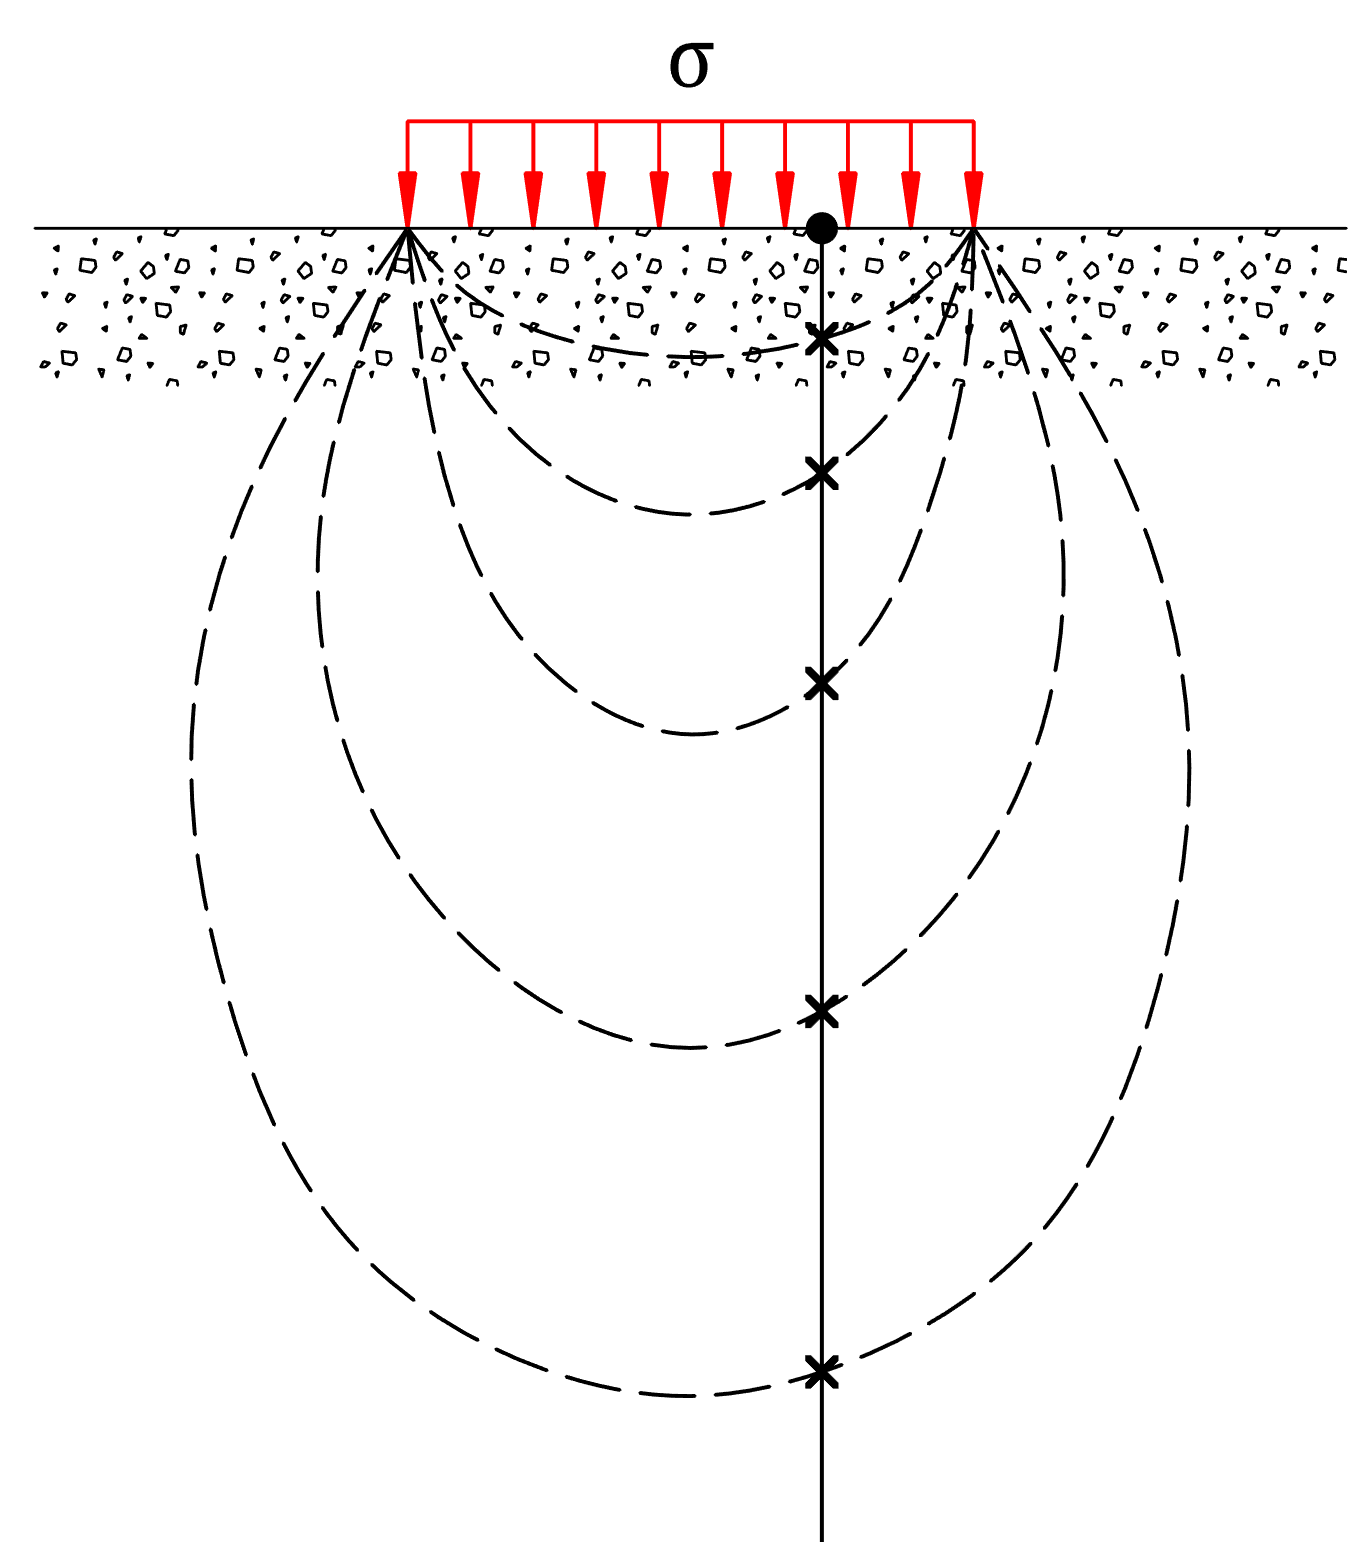
\includegraphics[width=0.5\linewidth,keepaspectratio]{papers/spannung/Grafiken/Bild4.png}
	\caption{Ausbreitung der Spannung im Boden}
	\label{fig:Bild4}
\end{figure}

\begin{figure}
	\centering
	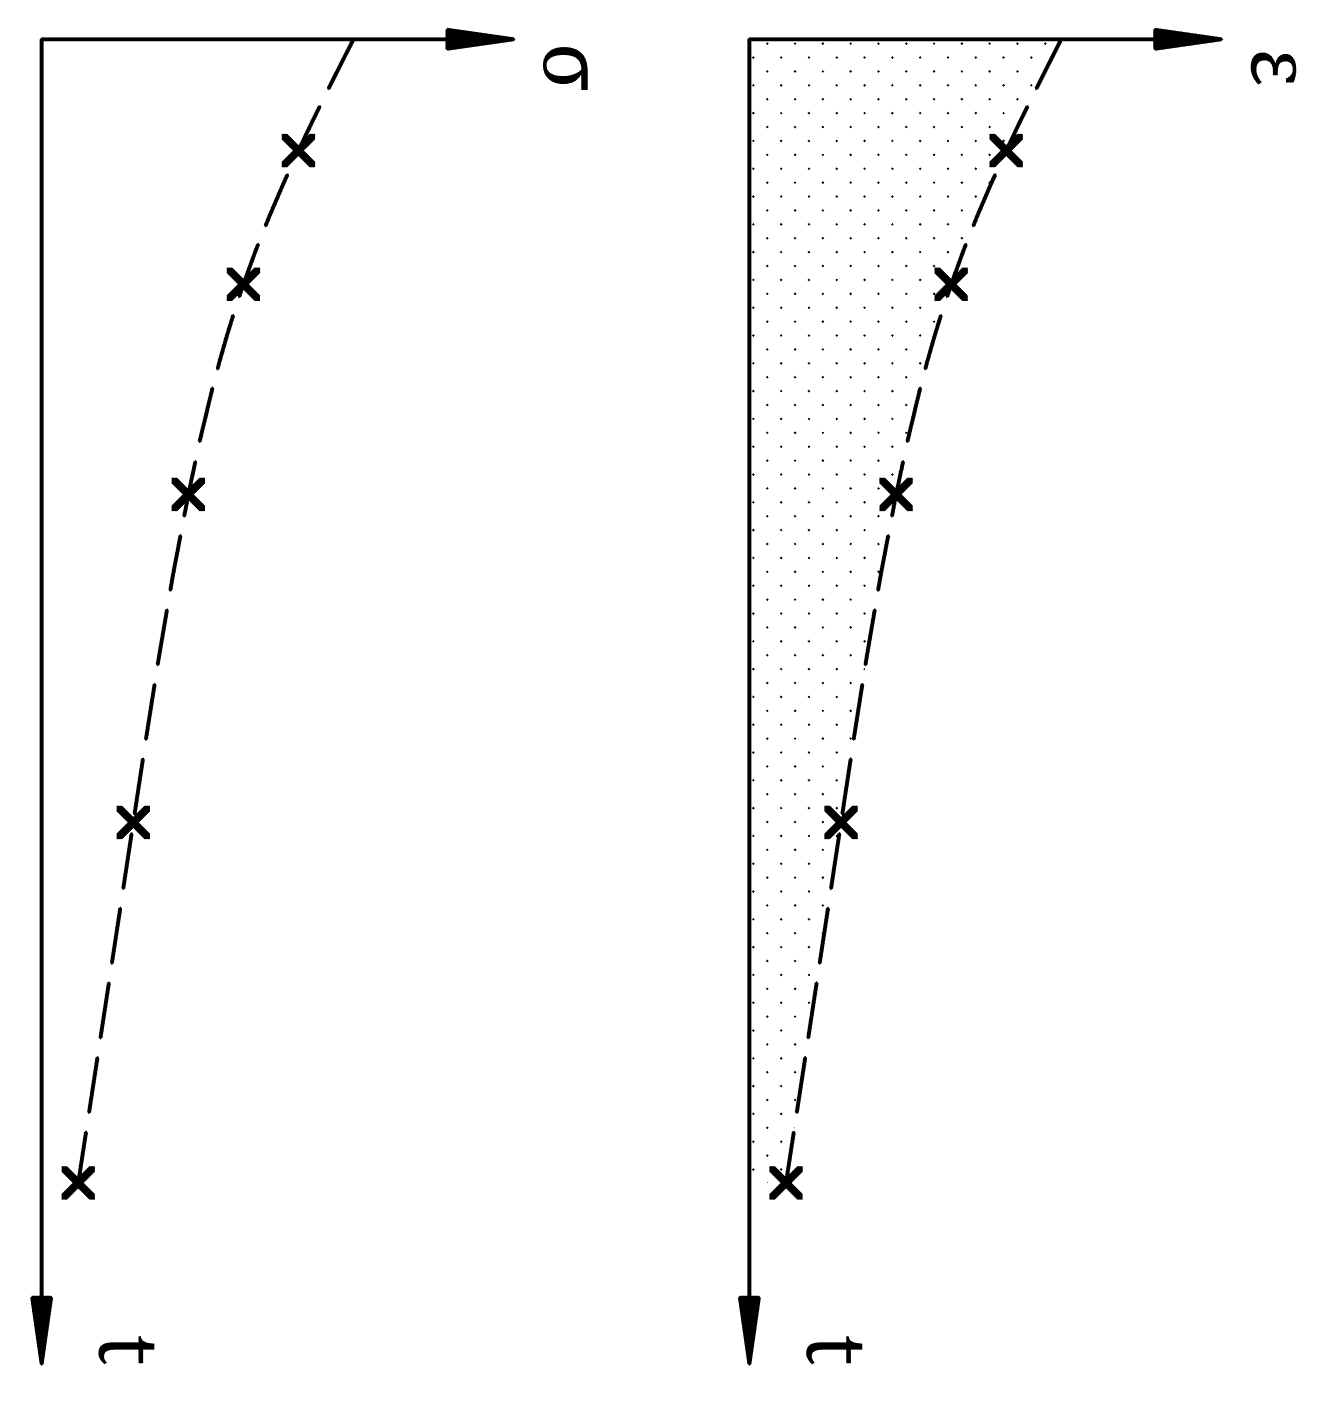
\includegraphics[width=0.5\linewidth,keepaspectratio]{papers/spannung/Grafiken/Bild5.png}
	\caption{Funktionen Spannung und Dehnung}
	\label{fig:Bild5}
\end{figure}

Anhand eines etwas schwierigeren Beispiels sieht man,
dass die Spannungsausbreitung nicht immer ganz einfach ist.
Man hat hier eine Baugrube mit einem Baugrubenabschluss, wo ein Teil des Bodens abgetragen wurde.
Was aber immer noch gilt ist, dass die Spannung $\sigma$ von drei Variablen abhängig ist $(x,y,t)$.
Ansätze um die Spannungsausbreitung zu berechnen gibt es je nach Bodentyp verschiedene.

\begin{figure}
	\centering
	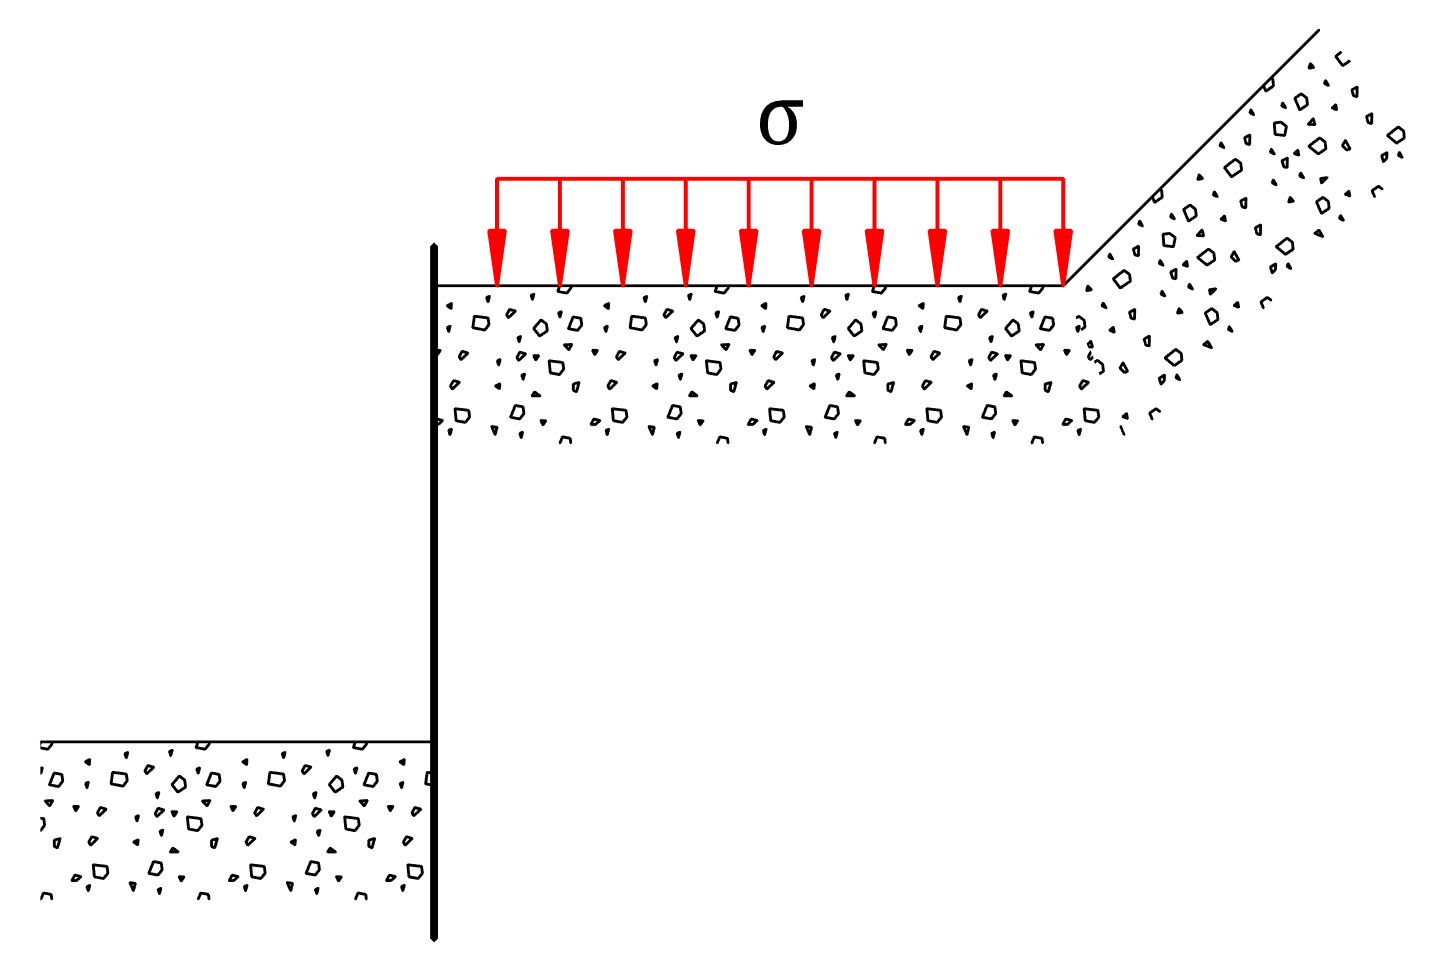
\includegraphics[width=0.5\linewidth,keepaspectratio]{papers/spannung/Grafiken/Bild3.png}
	\caption{Beispiel Lastauftrag auf Boden}
	\label{fig:Bild3}
\end{figure}

Die Spannungsausbreitung ist uns jedoch gegeben, es geht nicht darum, dies genauer zu untersuchen.
Durch die Spannungsausbreitung und das Elastizitätsmodul kann man eine Dehnung berechnen.
Anhand dieser Dehnung kann man mit einem Integral wiederum die Setzung berechnen.
\[
\varepsilon
=
\frac{\sigma}{E}
\]
\[
s
=
\int_{0}^{\infty}\varepsilon\enspace dt
\]
Die Setzung zu bestimmen ist in der Geotechnik sehr wichtig.
Besonders ungleichmässige Setzungen können bei Bauwerken Probleme ergeben.
Es gilt also die Bauwerke so zu dimensionieren, dass es verträgliche Setzungen gibt.